\chapter{Prostheses} \label{prostheses}
%\discuss{I think that this might be a bit off topic. it is really interesting, and awesome, but it might be more relevant to make an outline "one option for a prostheses would be bionic arms, they are generally such and such, and functions such and such. to add a comparison to normal plastic prostheses, to a normal arm and to robotic alternatives (something a bit more conventional? idk) we need this chapter to conclude that the robotic prostheses is the best option for us. this is difficult, since we don't have a problem defined yet >.<}
\section{Bionic end-effector}

Bionic prostheses is the closest a person with reduced functionality will come to a real arm.\\
In this chapter several options for bionic arms will be examined, to get a better understanding of the mechanics of the products on the market.\\

\subsection{I-limb Ultra}

\begin{figure}[H]
    \centering
    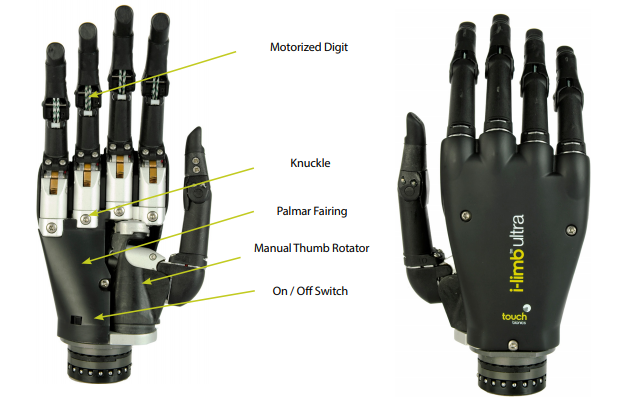
\includegraphics[width=12cm]{Sections/Contextual_Analysis/ProsthesesPics/i-limbultra.png}
    \caption{I-Limb Ultra\cite{I-limbUltra}}
    \label{fig:Ilimb-Ultra}
\end{figure}

The I-Limb Ultra device is an attachable bionic hand. It's flexible architecture allows the patient to use both apps and muscles to signal the grip. The myoelectric signals from sensors in the patients residual limbs allows the hand to move as desired, while the app is for quick controls and specific grips.\\
The device has implemented proximity control administered by small Bluetooth devices, which triggers a grip when the the device is close to an object.\\
Gesture control is another feature offered by the "I-limb quantum". This allows the user to move the device in a certain direction to trigger a special and customizable grip \cite{I-limbUltra}.

\begin{figure}[H]
    \centering
    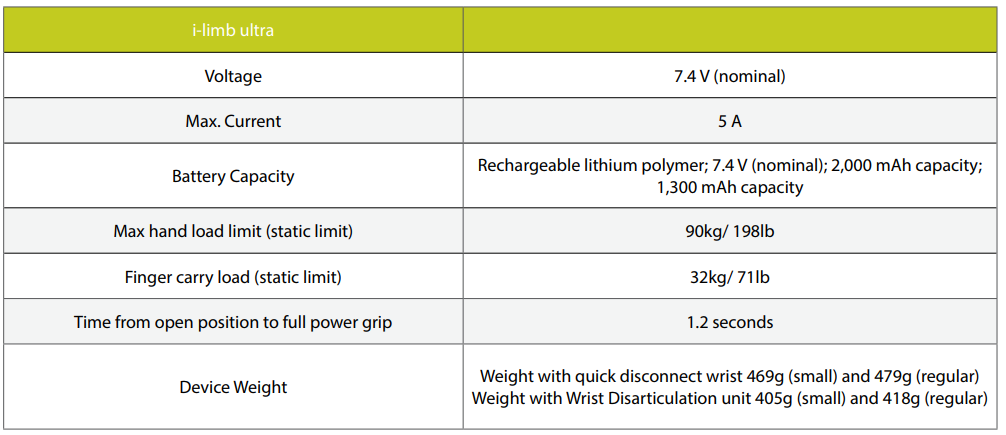
\includegraphics[width=15cm]{Sections/Contextual_Analysis/ProsthesesPics/specs.png}
    \caption{I-Limb Ultra Specifications\cite{I-limbUltra}}
    \label{fig:Ilimb-UltraSpecs}
\end{figure}
\clearpage

\subsection{Be-Bionic}

\begin{figure}[H]
    \centering
    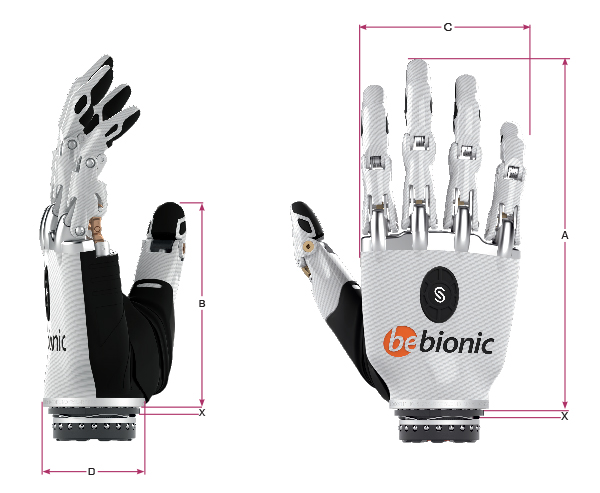
\includegraphics[width=10cm,height=7cm]{Sections/Contextual_Analysis/ProsthesesPics/Be-bionic.jpg}
    \caption{Be-Bionic \cite{Be-bionic}}
    \label{fig:Be-Bionic}
\end{figure}

The Be-Bionic hand take advantage of multiple ergonomic features. The weight distribution of the motors in hand makes the hand more comfortable and feel lighter.\\
Balance software and microprocessors implemented in the hand, monitors the position and gives a more precise control.\\
Another useful feature is the auto grip, that ensures when items is slipping, the hand will then readjust to prevent that happening.\\

\begin{figure}[H]
    \centering
    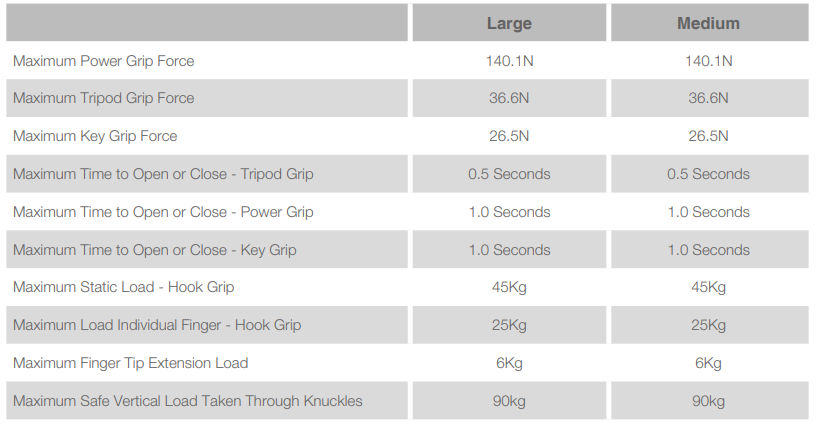
\includegraphics[width=15cm,height=6cm]{Sections/Contextual_Analysis/ProsthesesPics/specs-bebionic.png}
    \caption{Be-Bionic Specifications \cite{Be-bionic}}
    \label{fig:Be-BionicSpecs}
\end{figure}
